\begin{figure}[H]
    \centering
    \definecolor{profileblue}{RGB}{35,105,180}
    \definecolor{midred}{RGB}{185,45,45}
    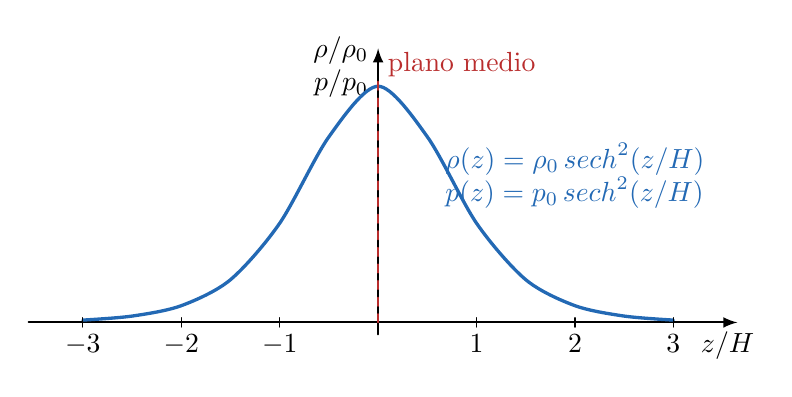
\begin{tikzpicture}[x=1.25cm,y=3.0cm,line cap=round,line join=round]
        % Ejes adimensionales
        \draw[-latex,line width=0.75pt] (-3.55,0) -- (3.65,0);
        \draw[-latex,line width=0.75pt] (0,-0.05) -- (0,1.16);
        \node[below] at (3.55,0) {$z/H$};
        \node[left,align=right] at (0,1.08)
            {$\rho/\rho_0$\\$p/p_0$};

        % Perfil sech^2
        \draw[profileblue,line width=1.2pt,smooth]
            plot coordinates {
                (-3,0.010) (-2.5,0.027) (-2,0.071)
                (-1.5,0.181) (-1,0.420) (-0.5,0.786)
                (0,1.000)
                (0.5,0.786) (1,0.420) (1.5,0.181)
                (2,0.071) (2.5,0.027) (3,0.010)
            };

        \draw[midred,dashed,line width=0.7pt] (0,0) -- (0,1.02);
        \node[midred,above right] at (0,1.00) {plano medio};
        \node[profileblue,align=left] at (2.00,0.62)
            {$\rho(z)=\rho_0\,\operatorname{sech}^2(z/H)$\\
             $p(z)=p_0\,\operatorname{sech}^2(z/H)$};

        \foreach \x in {-3,-2,-1,1,2,3} {
            \draw (\x,0.02) -- (\x,-0.02);
            \node[below] at (\x,-0.01) {$\x$};
        }
    \end{tikzpicture}
    \caption{Perfiles normalizados de densidad y presión de la placa isotérmica.}
\end{figure}